% Version française de « Normative Trees: Selecting the Applicable Rule in
% French Labour Law » (soumission JURIX 2026), mise au format des JFLA.
% Version bis : exemple fil rouge tiré du corpus Catala, architecture
% d'A-Lex, figures, opérateur de point de choix.



\documentclass[review]{jflart}
\usepackage[utf8]{inputenc}
\usepackage[T1]{fontenc}
\usepackage{normtrees-fr}
\usepackage{fancyvrb}
\usepackage{tikz}
\usetikzlibrary{arrows.meta,babel}
\colorlet{elague}{black!40}

% Notations ajoutées dans la version bis
\newcommand{\ALex}{A-Lex}
\newcommand{\Brancher}{\ensuremath{\mathsf{Brancher}}}
\newcommand{\conflit}{\mathbin{\#}}
\newcommand{\Conf}{\ensuremath{\mathsf{Conf}_D}}
\newcommand{\Categorie}{\ensuremath{\mathsf{Categorie}}}
\newcommand{\Cadre}{\ensuremath{\mathsf{IngenieurOuCadre}}}
\newcommand{\Etam}{\ensuremath{\mathsf{Etam}}}
\newcommand{\Presence}{\ensuremath{\mathsf{AnneesDePresence}}}
\newcommand{\MoisRem}{\ensuremath{\mathsf{MoisDeRemuneration}}}
\newcommand{\MatJ}{\ensuremath{\mathsf{MatiereJuridique}}}
\newcommand{\refine}{\mathrel{\twoheadrightarrow}}
\newcommand{\Ouv}{\ensuremath{\mathit{Ouv}}}
\newcommand{\ModeRupture}{\ensuremath{\mathsf{ModeRupture}}}
\newcommand{\PreavisNE}{\ensuremath{\mathsf{PreavisNonExecute}}}
\newcommand{\IndemRupture}{\ensuremath{\mathsf{IndemniteDeRupture}}}


\jfla{38}{2027}

\title{Arbres normatifs : déterminer la règle applicable en droit du travail
  français}
\titlerunning{Arbres normatifs et règle applicable en droit du travail}

\author[1,2]{Guel Faure}
\author[2]{Jean Krivine}
\author[1,3]{Eïtan Carta-Lag}
\authorrunning{Faure, Krivine et Carta-Lag}

\affil[1]{LUMO (SARL), Grenoble, France}
\affil[2]{Université Paris Cité, CNRS, IRIF, F-75013, Paris, France}
\affil[3]{Acquis De Droit (cabinet d'avocats), Grenoble, France}

\begin{document}

\maketitle

\begin{abstract}
  En droit du travail français, un calcul tel que celui de l'indemnité légale
  de licenciement ou de la durée d'un préavis commence avant l'arithmétique :
  il faut d'abord déterminer quelle règle est juridiquement habilitée à fournir
  la formule. Pour une matière juridique donnée, plusieurs textes, ou plusieurs
  versions temporelles d'un même texte, peuvent proposer des fonctions
  concurrentes, et la manière dont elles s'articulent dépend du régime
  d'articulation applicable. Nous modélisons cette couche de sélection de la
  règle comme un processus de résolution déterministe, destiné à assister les
  experts juridiques. Nous l'illustrons sur un exemple tiré d'un corpus de droit
  du travail écrit en Catala, et l'étendons par des valeurs en conflit et un
  opérateur de branchement, qui construisent des demandes principales et
  subsidiaires. Ce
  modèle fournit l'architecture de l'assistant A-Lex.
\end{abstract}

\section{Introduction}\label{sec:introduction}

Supposons qu'une salariée demande quelle indemnité lui serait due en cas de
licenciement, ou souhaite connaître la durée de son préavis. Même si toutes les
formules candidates qui représentent fidèlement le droit français sont
exécutables, la réponse ne peut se réduire à un nombre, ni même à une fonction.
La question préalable est : \emph{quelle règle juridique est applicable à cette
salariée, pour cette question, à la date juridiquement pertinente ?} Un
assistant doit donc identifier le texte dont procède la règle, l'état de ce
texte dans le temps et les faits qui permettent d'entrer dans sa branche, tout
en conservant, pour contrôle, les alternatives écartées et le fondement de la
sélection.

Le droit du travail français rend cette question particulièrement visible, car
ses sources ne s'articulent pas selon une hiérarchie monotone unique. L'ordre
public absolu exclut toute dérogation contractuelle ou conventionnelle, même
plus favorable ; l'ordre public social permet d'améliorer le socle légal en
vertu du principe de faveur ; l'ordre public dérogatoire, ou les dispositions
supplétives, autorisent des dérogations négociées dans un champ défini par le
législateur~\cite{viepublique2021}. Le calcul en cause doit donc être identifié
avant que la hiérarchie des sources puisse sélectionner une règle. Ainsi,
l'article L2253-1 du \emph{Code du travail} dispose :
\begin{quote}\itshape
  Dans les matières énumérées au 1° à 13°, les stipulations de la convention de
  branche ou de l'accord couvrant un champ territorial ou professionnel plus
  large prévalent sur la convention d'entreprise conclue antérieurement ou
  postérieurement à la date de leur entrée en vigueur, sauf lorsque la
  convention d'entreprise assure des garanties au moins équivalentes. [\dots]
\end{quote}
Cette disposition illustre comment un texte peut empêcher qu'un calcul fourni
par une source de rang supérieur soit écarté par une source de rang inférieur
lorsque celle-ci produirait un résultat moins favorable. À l'inverse,
l'article L2253-3 dispose :
\begin{quote}\itshape
  Dans les matières autres que celles mentionnées aux articles L. 2253-1 et
  L. 2253-2, les stipulations de la convention d'entreprise conclue
  antérieurement ou postérieurement à la date d'entrée en vigueur de la
  convention de branche ou de l'accord couvrant un champ territorial ou
  professionnel plus large prévalent sur celles ayant le même objet prévues par
  la convention de branche ou l'accord couvrant un champ territorial ou
  professionnel plus large. En l'absence d'accord d'entreprise, la convention
  de branche ou l'accord couvrant un champ territorial ou professionnel plus
  large s'applique.
\end{quote}
Pour ces autres matières, l'accord d'entreprise, s'il existe, écarte l'accord
de branche ; à défaut, ce dernier demeure la règle de repli~\cite{frarticulation}.
Ce schéma de priorité est issu de la réforme de 2017, qui a renforcé la
négociation d'entreprise dans les champs fixés par la
loi~\cite{viepublique2017}.

Notre question de recherche est la suivante : \emph{comment un assistant
juridique peut-il organiser et résoudre des calculs concurrents de droit du
travail, identifier les informations nécessaires à leur sélection, et conserver
explicites et contrôlables les choix qui en résultent, afin d'aider un expert
juridique, éventuellement un grand modèle de langage (LLM), à construire une
plaidoirie sur une base maîtrisée et transparente ?} Nous apportons plusieurs
contributions en ce sens. Premièrement, nous définissons des \emph{candidats}
typés par matière et indexés par leur source, représentants formels des textes
juridiques qui définissent un calcul, et nous précisons comment ce calcul se
comporte vis-à-vis des textes relatifs à la même matière mais situés à un
niveau inférieur. Deuxièmement, nous organisons ces objets formels en
\emph{forêts normatives} ordonnées par les sources et à arêtes prédicatives,
qui représentent à la fois les dépendances hiérarchiques entre candidats et les
conflits qui les opposent ; nous organisons de même les matières en une
\emph{hiérarchie} de raffinement conditionnel, qui assure que les candidats
d'un même arbre portent sur une même matière concrète. Troisièmement, nous montrons comment une boucle
interactive assiste l'expert juridique dans la sélection et le calcul du droit
applicable, et nous l'étendons aux valeurs en conflit : lorsqu'un fait ou une
qualification est discuté, l'utilisateur en donne plusieurs valeurs ordonnées,
et un opérateur de \emph{branchement} crée un scénario par valeur, pour
ordonner des demandes principales et subsidiaires. Un exemple fil rouge, tiré
d'un corpus de droit du travail écrit en Catala, accompagne chaque étape
(section~\ref{sec:exemple}).

\paragraph{Architecture d'\ALex{}.}
Ce modèle fournit l'architecture d'\ALex{}, l'assistant juridique que nous
développons. \ALex{} exécute un corpus de droit du travail écrit en
Catala~\cite{merigoux2021,corpuslumo}, dans lequel chaque source, le Code du
travail ou une convention collective, est un module qui rend sa propre réponse
à une même question. Les modules des sources ne comparent pas leurs réponses :
la comparaison sous l'ordre public social relève d'un module de concours
distinct, et le régime d'articulation qui décide du concours à mener n'est pas
encodé : le corpus le laisse, à dessein, hors du code. Ce régime est porté ici
par les politiques d'arbitrage des candidats, que la forêt normative organise.
Les notions introduites ici organisent les composants du prototype d'\ALex{}. Un indexeur lit les modules
Catala et en extrait les candidats ; un moteur d'élagage construit la forêt exhaustive,
la réduit au dossier et formule les questions à poser ; la sélection finale
applique les politiques d'arbitrage aux valeurs que calcule le code Catala
compilé ; un gestionnaire de scénarios enregistre les valeurs en conflit et en
tire les demandes subsidiaires.

Notre contribution est délibérément circonscrite : elle ne prétend pas saisir
toutes les caractéristiques du droit du travail, et elle ne traite pas le
problème de la traduction de textes juridiques rédigés en langue naturelle en
fonctions calculables qui les implémentent fidèlement.

\section{Exemple fil rouge}\label{sec:exemple}

\paragraph{Le dossier.}
Une salariée d'une société de conseil relevant de la convention collective
Syntec (IDCC~1486) reçoit, en mars 2025, la notification de son licenciement,
qui n'est pas prononcé pour faute grave. Elle compte dix ans d'ancienneté et
son salaire de référence est de 3\,000 euros. Sa classification est discutée :
son employeur la range parmi les ETAM (employés, techniciens et agents de
maîtrise) ; elle soutient relever des ingénieurs et cadres. Elle demande ce
qui lui est dû au titre de la rupture. Le dossier initial contient la date de
la notification, le mode de rupture, l'exécution du préavis, l'ancienneté et le
salaire de référence ; la convention applicable et la catégorie restent à
établir.

\paragraph{Les textes en Catala.}
Nous reprenons les textes tels que les écrit le corpus~\cite{corpuslumo}, où
chaque bloc de code est placé sous l'article qu'il traduit ; la
figure~\ref{fig:catala} en reproduit deux extraits. L'article R.~1234-2 du Code
du travail, dans sa version en vigueur depuis le 27~septembre 2017, fixe le
montant plancher : un quart de mois de salaire par année d'ancienneté jusqu'à
dix ans, un tiers au-delà~\cite{frcode}. L'article 4.5 de la convention Syntec,
en vigueur depuis le 1\textsuperscript{er}~mai 2023, fixe un barème propre, qui
distingue les ETAM des ingénieurs et cadres~\cite{syntec} ; avant cette date,
l'article~19 de la convention s'appliquait.

\begin{figure}
\begin{Verbatim}[frame=single, label={Code du travail, article R. 1234-2}]
champ d'application MontantIndemnitéDeLicenciement_Loi:
  étiquette plancher_légal_r1234_2
  définition montant_du_plancher
    sous condition années_ancienneté <= 10,0
    conséquence égal à
      montant_du_salaire_de_référence * années_ancienneté * (1,0 / 4,0)

  étiquette plancher_légal_r1234_2
  définition montant_du_plancher
    sous condition années_ancienneté > 10,0
    conséquence égal à
      montant_du_salaire_de_référence * 10,0 * (1,0 / 4,0)
      + montant_du_salaire_de_référence * (années_ancienneté - 10,0)
        * (1,0 / 3,0)
\end{Verbatim}
\begin{Verbatim}[frame=single, label={Convention Syntec (IDCC 1486), article 4.5}]
champ d'application MontantIndemnitéDeLicenciement_CCN_1486
  sous condition
    article_4_5_applicable_VersionApplicableRuptureDuContrat_CCN_1486:
  étiquette barème
  définition montant_du_barème
    sous condition
      faits_rupture.catégorie = Etam
      et années_de_présence <= 10,0
    conséquence égal à
      mois_de_rémunération * années_de_présence * (1,0 / 4,0)

  étiquette barème
  définition montant_du_barème
    sous condition
      faits_rupture.catégorie = IngénieurOuCadre
      et années_de_présence >= 2,0
    conséquence égal à
      mois_de_rémunération * années_de_présence * (1,0 / 3,0)
\end{Verbatim}
\caption{Deux extraits du corpus Catala~\cite{corpuslumo} : le barème légal et
  le barème conventionnel de l'indemnité de licenciement. Commentaires omis et
  mise en page adaptée ; les deux autres cas du barème Syntec (ETAM au-delà de
  dix ans, cadres de moins de deux ans) sont omis.}
\label{fig:catala}
\end{figure}

Chaque champ d'application calcule la réponse de sa source, et rien d'autre.
Deux informations manquent au code pour conclure : la source qui doit
l'emporter, et le régime qui en décide. Le corpus les laisse hors du code, à
dessein : sous les articles R.~1234-1 et R.~1234-2, un commentaire indique que
la formule « ne peut être inférieure » fait du barème légal un minimum d'ordre
public social, qualification que le code n'encode pas, et que la comparaison
avec une source plus favorable relève d'un module distinct. Les étiquettes et exceptions
internes à un texte, comme le barème par catégorie ou l'exclusion de la faute
grave, restent au contraire dans le code Catala.

\paragraph{Ce que l'assistant doit établir.}
L'assistant doit d'abord préciser la question : ici, le licenciement fait de
l'indemnité de licenciement la matière en cause. Trois questions se posent
ensuite : quelle convention collective s'applique, quelle version de cette
convention régit la date de la notification, et dans quelle catégorie ranger
la salariée. Les sections suivantes reprennent ce dossier à chaque étape :
matières et candidats (section~\ref{sec:notations}), hiérarchie des matières et
arbre normatif (section~\ref{sec:forest}, figures~\ref{fig:hierarchie}
et~\ref{fig:arbre}), élagage, faits requis, sélection finale et branchement
sur la catégorie (section~\ref{sec:op}).

\section{Travaux connexes et positionnement}\label{sec:related}

\paragraph{Règles juridiques exécutables.}
Les travaux dits \emph{Rules as Code} étudient l'évaluation, la représentation
et l'exécution disciplinées des dispositions juridiques~\cite{ali2025}.
LegalRuleML structure règles, sources, exceptions et
métadonnées~\cite{nazarenko2016,legalruleml} ; L4 dote les contrats d'une
sémantique d'exécution déontique et temporelle~\cite{watt2023} ; Catala modélise
les règles par défaut et les exceptions de la loi~\cite{merigoux2021}. Le présent
travail commence là où ce problème est supposé résolu : les textes juridiques
y sont représentés par des objets formels qui contiennent la partie
calculatoire du droit. On fait abstraction du langage formel utilisé
concrètement pour implémenter ces fonctions.

\paragraph{Gestion des exceptions dans Catala.}
Catala résout les définitions concurrentes d'une variable par une logique des
défauts à priorités~\cite{merigoux2021} : la sélection dépend de conditions
d'applicabilité et d'un ordre statique entre exceptions, jamais des valeurs que
produiraient les définitions. Le principe de faveur dépend au contraire du
résultat ; l'encoder par le mécanisme des exceptions impose de conditionner
une exception à une comparaison de valeurs placée dans le texte inférieur, pour
chaque paire de sources. Le corpus de la section~\ref{sec:exemple} l'évite en
écrivant la comparaison dans un module de concours distinct
(figure~\ref{fig:concours}), ce qui revient, comme ici, à sortir le principe de
faveur des textes eux-mêmes. Les arbres normatifs attachent la politique au candidat supérieur,
fixent une fois pour toutes l'ordre de favorabilité de chaque matière, et
procèdent par un \emph{fold} uniforme le long du chemin des sources. Les deux
approches sont complémentaires : Catala structure les exceptions au sein d'un
texte ; les arbres normatifs articulent des textes concurrents.

\paragraph{Raisonnement défaisable et conflits de normes.}
Les conflits entre normes sont classiquement traités par des règles
défaisables munies d'une relation de priorité, elle-même éventuellement
dérivée par des règles~\cite{prakkensartor1996,prakkensartor1997}, et par des
logiques défaisables dans lesquelles \emph{lex superior}, \emph{lex specialis}
et \emph{lex posterior} instancient la relation de
supériorité~\cite{governatori2021} ; les versions temporelles d'un texte y sont
traitées comme des modifications de normes~\cite{governatori2005}. Les arbres
normatifs s'en distinguent sur trois points. D'abord, la priorité n'est pas une
propriété du couple de normes mais de la norme supérieure, qui énonce comment
elle tolère les sources inférieures ; \emph{lex superior} (\(\Absolute\)), son
inverse (\(\Suppletive\)) et le principe de faveur, qui dépend du résultat
(\(\Social\)), coexistent ainsi le long d'un même chemin. Ensuite, la sélection
sous \(\Social\) exige d'évaluer les deux candidats, ce que des priorités
statiques ou dérivées par des règles n'expriment pas. Enfin, un fait manquant
bloque la résolution et engendre une demande, au lieu de laisser une règle
s'appliquer par défaut. En contrepartie, la portée est plus étroite : candidats
d'une seule matière, frères mutuellement exclusifs plutôt qu'une relation
générale de spécificité, et politiques non encore dérivées de textes tiers
(section~\ref{sec:conclusion}).

\paragraph{Modèles du raisonnement juridique.}
Plusieurs approches modélisent le raisonnement juridique comme un processus
structuré de construction et de résolution d'arguments
juridiques~\cite{gordon1993pleadings,benchcapon2009argumentation}. Notre travail
s'y rattache tout en étant délibérément plus étroit : il automatise
partiellement les parties de ce processus gouvernées par des calculs
formalisés, des conditions d'applicabilité et des politiques d'arbitrage. Les
jugements interprétatifs et stratégiques de l'expert juridique sont représentés
abstraitement par \(\Input\) et par les valeurs en conflit
(section~\ref{sec:choix}), tandis que leurs conséquences pour l'élagage, la
sélection et l'exécution restent explicites et contrôlables.

\section{Notations et terminologie}\label{sec:notations}

\begin{defi}[Matières et domaines de valeurs]\label{def:types}
Une \emph{matière} \(m\in\Matter\) est une question juridique nommée. Elle
est \emph{concrète} lorsqu'elle désigne une grandeur juridique déterminée, par
exemple \(\Salary\), \(\Senior\), \(\Indem\), \(\IndemLeg\), \(\IDCC\) ou
\(\DateT\), et \emph{abstraite} lorsqu'elle regroupe des matières qui la
précisent, comme l'indemnité de rupture \(\IndemRupture\), que le mode de
rupture précise en indemnité de licenciement ou en indemnité compensatrice de
préavis. On note \(\Matter_c\) l'ensemble des matières concrètes. Chaque
matière concrète possède un \emph{domaine de valeurs} \(\Raw(m)\), l'ensemble
de ses valeurs brutes possibles :
\[
\begin{array}{c}
 \Raw(\Salary)=\Raw(\Indem)=\Raw(\IndemLeg)=\Money,\\
 \Raw(\Senior)=\Duration,\quad
 \Raw(\DateT)=\mathsf{Date},\quad
 \Raw(\IDCC)=\mathbb N
\end{array}
\]
où \(\Money\) et \(\Duration\) désignent les montants et les durées. Des
matières distinctes peuvent partager un même domaine : \(\Indem\) et \(\Salary\)
sont toutes deux des montants, mais ce sont des grandeurs juridiques
différentes, et les fonctions juridiques (définition~\ref{def:rule-package})
sont typées par les matières, non par les domaines. La matière \(\IDCC\) est un
identifiant, qui détermine la convention collective applicable.
\end{defi}

Seules les matières concrètes reçoivent des valeurs ; une matière abstraite
pose une question que le dossier précise, selon une hiérarchie définie à la
section~\ref{sec:hierarchie} une fois introduits les prédicats
d'applicabilité.

\begin{defi}[Ordre de favorabilité]\label{def:favorable}
Une matière concrète \(m\) peut être munie d'un ordre total \(\fav{m}\) sur
\(\Raw(m)\) ;
on lit \(x\fav{m}y\) : « \(y\) est au moins aussi favorable au salarié
que~\(x\) », et \(x\strictfav{m}y\) désigne sa partie stricte. Le sens de
l'ordre dépend de la matière :
\(\fav{\Indem}=\mathord{\leq}\),
\(\fav{\mathsf{RetenueSurSalaire}}=\mathord{\geq}\), et
\(\false\strictfav{\mathsf{Indemnisable}}\true\).
\end{defi}

On note \(\MatterOrd\subseteq\Matter_c\) les matières munies d'un tel ordre.
Seules ces matières admettent des candidats de politique \(\Social\), ce
qu'impose la cohérence (section~\ref{sec:consistency}) ; la comparaison porte
sur les valeurs que les candidats concurrents produisent pour le dossier
considéré, et non sur les textes eux-mêmes.

\paragraph{Exemple.} La demande de la salariée porte sur la matière abstraite
\(\IndemRupture\). Le dossier fil rouge met en jeu les matières concrètes
\[
\begin{array}{c}
\Indem,\ \Senior,\ \Salary,\ \Presence,\ \MoisRem,\\
\IDCC,\ \DateT,\ \ModeRupture,\ \PreavisNE\ \text{et}\ \Categorie,\\
\text{avec}\quad\{\Etam,\Cadre\}\subseteq\Raw(\Categorie),
\end{array}
\]
et l'indemnité est munie de l'ordre \(\fav{\Indem}=\mathord{\leq}\) sur les
montants. L'ancienneté et le salaire au sens de la convention, \(\Presence\) et
\(\MoisRem\) dans le code de la figure~\ref{fig:catala}, sont des matières
distinctes de leurs homologues légales : le corpus les calcule séparément, et
elles valent ici dix ans et 3\,000 euros elles aussi.

\begin{defi}[Dossier]\label{def:dossier}
Un dossier \(D\) est donné par un couple
\(D:=(\mathcal M_D,\nu_D)\in\Dossier\), où \(\mathcal M_D\subseteq\Matter_c\)
est l'ensemble des matières concrètes soulevées par le dossier et \(\nu_D\) sa
valuation courante :
\[
\nu_D:\prod_{m\in\mc M_D}\left(\Raw(m)\uplus\mc T(m)\right).
\]
\end{defi}

La valuation attribue à chaque matière exactement l'un des deux états suivants. Une
matière est \emph{résolue} lorsque \(\nu_D\) lui associe une valeur brute, et
\emph{non résolue} lorsque \(\nu_D\) lui associe l'arbre normatif qu'il reste à
résoudre. Une matière \(m\in\Matter_c\setminus\mc M_D\) est \emph{indéfinie}
dans~\(D\). Ainsi
\[
\begin{aligned}
\Res&:=\{m\in\mathcal M_D\mid \nu_D(m)\in\Raw(m)\},\\
\Unres&:=\{m\in\mathcal M_D\mid \nu_D(m)\in\mc T(m)\},\\
\Undef&:= \{m\in\Matter_c \mid m\not\in \mc M_D\}.
\end{aligned}
\]

\begin{defi}[Sources juridiques et ordre normatif]\label{def:source-order}
Les sources juridiques forment un ensemble partiellement ordonné
\((\Source,\normge)\), où \(\normge\) modélise l'\emph{ordre normatif}. La
relation stricte \(s\normgt s'\) signifie que la source \(s\) est au-dessus de
la source \(s'\) dans la hiérarchie des sources. On note
\(\normdown(s):=\{s'\in\Source\mid s'\normlt s\}\).
\end{defi}

L'ensemble \(\Source\) est interprété comme le type sommet de la relation de
sous-typage \({\subtype}\subseteq\Source\times\Source\), qui classe les sources
selon la taxonomie en usage en droit du travail français. On emploie parfois
\(s\in\Source\) comme synonyme de \(s\subtype\Source\). Par exemple
\[
\CodeTravail\subtype\Source,\quad
\AccordCollectif\subtype\Source,\quad
\Contrat\subtype\Source,
\]
et, pour tout type \(s\) parmi \(\AccordInterpro\), \(\ConvBranche\) et
\(\AccordEntreprise\), on a \(s\subtype\AccordCollectif\). La relation de sous-typage ne doit pas être
confondue avec l'ordre normatif. Pour tous \(s_i\in\Source\), on exige
\[
\begin{array}{rll}
s_0\normlt s_1&\implies& {s_0 \not\subtype s_1} \wedge {s_1\not\subtype s_0}\\
{s_0\subtype s_1}\wedge {s_1\normlt s_2}\wedge {s_3\subtype s_2}& \implies &s_0\normlt s_3\quad \text{(clôture par sous-typage)}
\end{array}
\]

\begin{defi}[Fonction juridique]\label{def:rule-package}
Une fonction juridique encode la partie calculatoire d'un texte juridique. On
la note \(f\in\Fun\) ; c'est un couple \(f=(\sigma_f,\phi_f)\) où, pour
\(n\in\mathbb N\) et \(m_0,\ldots,m_n,m\in\Matter_c\),
\[
 \sigma_f=(m_0,\ldots,m_n)\longrightarrow m,
 \qquad
 \phi_f:\prod_{i=0}^{n}\Raw(m_i)\longrightarrow\Raw(m).
\]
On note \(\Fun_m:=\{f\in\Fun\mid\exists \vec m:\sigma_f=\vec m\to m\}\)
l'ensemble des fonctions juridiques qui produisent la matière~\(m\).
\end{defi}

Ici \(\sigma_f\) est l'interface typée complète de \(f\), et \(\phi_f\) son
calcul ordinaire. Les matières d'entrée d'une fonction identifient exactement
les matières résolues du dossier dont elle a besoin.

\begin{defi}[Politique d'arbitrage et extension par sous-typage]\label{def:arbitration-policy}
Un \emph{régime d'articulation} (simplifié) est un élément de
\(
\Policy:= \{\Absolute, \Social, \Suppletive\}.
\)
Soit \(s \in \Source\) un type de source. Une \emph{politique d'arbitrage} pour
\(s\) est une fonction partielle finie
\[
  p :
  \normdown(s)
  \rightharpoonup
  \Policy .
\]
Pour tout \(t \in \normdown(s)\), soit
\[
  \Herit_{p}(t)
  :=
  \left\{
    p(T)
    \;\middle|\;
    T \in \operatorname{dom}(p)
    \text{ et }
    t \subtype T
  \right\}
\]
l'ensemble des régimes hérités par \(t\). La politique \(p\) est
\emph{cohérente pour le sous-typage} si
\(
  \left|\Herit_{p}(t)\right| \leq 1
\)
pour tout \(t \in \normdown(s)\).
L'\emph{extension par sous-typage} d'une politique \(p\) cohérente pour le
sous-typage est la fonction totale
\(
  \widehat{p} :
  \normdown(s)
  \longrightarrow
  \Policy \uplus \{\bot\}
\)
définie par
\[
  \widehat{p}(t)
  :=
  \begin{cases}
    \rho,
      & \text{si } \Herit_{p}(t)=\{\rho\},\\
    \bot,
      & \text{si } \Herit_{p}(t)=\varnothing.
  \end{cases}
\]
\end{defi}

Le type \(\Policy\) est une version simplifiée des régimes d'articulation : les
régimes dérogatoire et supplétif, qui obéissent au même schéma de sélection,
sont ici réunis sous \(\Suppletive\).

\begin{defi}[Texte juridique et interprétation candidate]\label{def:candidate}
Un texte juridique qui constitue une interprétation candidate pour une matière
non résolue est modélisé par un triplet \(c=(s,f,p)\in\Cand\), avec
\[
 \Cand \subseteq \{(s,f,p) \mid s\in\Source,\ f\in\Fun,\ p: \normdown(s)\rightharpoonup \Policy \}.
\]
Ses projections sont \(s(c)=s\), \(f(c)=f\) et \(p(c)=p\). On dit que le
candidat \(c\) est de matière \(m\) lorsque \(f(c)\in\Fun_m\)
(définition~\ref{def:rule-package}). La matière identifie la sortie produite par
le calcul, tandis que la source identifie le corpus juridique qui l'autorise.
La fonction partielle \(p\) est une politique d'arbitrage cohérente pour le
sous-typage (définition~\ref{def:arbitration-policy}). On note
\(\sigma_c:=\sigma_{f(c)}\), \(\phi_c:=\phi_{f(c)}\) et
\(\Cand_m:=\{c\in\Cand\mid f(c)\in\Fun_m\}\).
\end{defi}

La politique d'arbitrage \(p\) définit la manière dont \(c\) doit être comparé
aux candidats de la même matière situés plus bas dans l'ordre normatif. C'est
toujours l'extension \(\widehat p\) qui est utilisée en pratique (on note
\(\widehat p(c)\) l'extension de \(p(c)\)), et \(p\) doit se comprendre comme
une interprétation parcimonieuse du droit. Nous verrons que, pour un
candidat~\(c\) et une source \(s\normlt s(c)\), \(\widehat p(c)(s)=\Absolute\)
indique que \(c\) ne peut être remplacé par une autre interprétation \(c'\) dès
lors que \(s(c')\subtype s\). À l'inverse, \(\widehat p(c)(s)=\Suppletive\)
énonce que le candidat est remplacé par tout candidat \(c'\) tel que
\(s(c')\subtype s\). Enfin, une politique \(\Social\) énonce que \(c\) ne peut
être remplacé par un candidat issu d'une source inférieure que si cette
alternative fournit un calcul au moins aussi favorable, au sens de la
définition~\ref{def:favorable}. La sélection entre candidats au moyen des
politiques d'arbitrage fait l'objet de la définition~\ref{def:apply-policy}.

\paragraph{Exemple : du code Catala aux candidats.}
Chaque champ d'application du corpus qui répond à la question fournit un
candidat. Son code compilé est le calcul \(\phi_f\) ; les valeurs qu'il lit
d'autres champs, que le corpus déclare comme variables externes, forment
l'interface \(\sigma_f\) ; la condition de version qui garde le champ Syntec
(figure~\ref{fig:catala}) et le champ d'application de la convention deviennent
le prédicat de l'arête qui mène au candidat ; la politique, que le corpus
n'encode pas, est portée par le candidat. Le droit à l'indemnité étant supposé
ouvert, on obtient
\[
c_{\mathsf{Code}}=(\CodeTravail,\ f_{\mathsf{Code}},\ [\ConvBranche\mapsto\Social]),
\qquad
c_{4.5}=(\Syntec,\ f_{4.5},\ \emptyset),
\]
avec
\[
\begin{array}{l}
\sigma_{c_{\mathsf{Code}}}=(\Senior,\Salary)\to\Indem,\\
\sigma_{c_{4.5}}=(\Presence,\MoisRem,\Categorie)\to\Indem,
\end{array}
\]
et de même \(c_{19}\) pour l'article~19 de la convention. Le candidat du Code
porte la politique \(\Social\) envers les conventions de branche : c'est la
qualification que le corpus laisse hors du code.

\begin{remark}[Contraintes juridiques sur l'attribution des politiques]
La définition~\ref{def:candidate} permet délibérément de doter tout candidat de
n'importe quelle politique. Il s'agit d'une sur-approximation : une instance
juridiquement fidèle doit restreindre l'attribution des politiques selon les
règles qui gouvernent les sources et les matières
concernées~\cite{daugareilh2019sources}. Ces restrictions ne sont pas imposées
par la présente définition de \(\Cand\) ; elles relèvent de la validation
juridique d'une instance du modèle.
\end{remark}

\section{Arbres normatifs}\label{sec:forest}

\subsection{Tests d'applicabilité}

On fixe un ensemble \(\Tests\) de \emph{tests atomiques}, écrits chacun à
partir de constantes et de noms de matières. Pour un test \(t\),
\(\dep(t)\subseteq\Matter_c\) est l'ensemble fini des noms de matières qui
apparaissent dans \(t\). Un \emph{prédicat d'applicabilité} est une conjonction
finie \(t_1\land\cdots\land t_k\) de tests atomiques, avec
\(\dep(t_1\land\cdots\land t_k):=\bigcup_i\dep(t_i)\).

On utilise la logique trivaluée \(\Bthree:=\{\true,\false,\unknown\}\), dont les
valeurs signifient respectivement établi, exclu et actuellement inconnu, avec
les connecteurs forts de Kleene~\cite{kleene1952introduction} : pour la
conjonction, \(\false\) l'emporte sur \(\unknown\), qui l'emporte
sur~\(\true\).

\begin{defi}[Sémantique des tests]\label{def:applicability-predicate}
Étant donné un dossier \(D=(\mc M_D,\nu_D)\), la valuation partielle
\[
 \widehat \nu_D(m):=
 \begin{cases}
  \nu_D(m),&m\in\Res,\\
  \bot,&m\in\Unres\cup\Undef,
 \end{cases}
\]
s'étend en une évaluation \(\sem{\cdot}_D:\Tests\to\Bthree\) qui renvoie
\(\unknown\) dès que l'un de ses arguments vaut \(\bot\), et sinon la valeur
booléenne ordinaire du test (par exemple \(\sem{\IDCC=1486}_D=\unknown\) lorsque
\(\IDCC\notin\Res\)). Un test \(t\) est \emph{total} lorsque
\(\dep(t)\subseteq\Res\) implique \(\sem{t}_D\in\{\true,\false\}\).
\end{defi}

\subsection{Hiérarchie des matières}\label{sec:hierarchie}

Une matière abstraite se précise en matières concrètes selon le dossier : la
salariée qui demande ce qui lui est dû au titre de la rupture pose une
question abstraite, que le mode de rupture précise. Une matière n'en précise
d'ailleurs une autre que sous condition : la prime de vacances de la convention Syntec n'est
une sous-matière de la prime que pour un salarié qui relève de cette
convention. Plutôt qu'un sous-typage statique des matières, analogue à celui
des sources (définition~\ref{def:source-order}), nous organisons donc les
matières en une hiérarchie dont les arêtes portent, comme celles des arbres
normatifs, des prédicats d'applicabilité.

\begin{defi}[Hiérarchie des matières]\label{def:hierarchie}
Une \emph{hiérarchie des matières} est un couple \((\refine,\eta)\) où
\((\Matter,\refine)\) est un graphe orienté acyclique fini, de racine unique
\(\MatJ\), et où \(\eta\) associe à chaque arête \(m\refine m'\) un prédicat
d'applicabilité \(\eta(m,m')\). L'arête \(m\refine m'\) signifie que \(m'\)
précise \(m\), ou en est un sous-cas, lorsque le dossier satisfait
\(\eta(m,m')\). Les matières sans successeur sont exactement les matières
concrètes. Comme pour les arbres, on pose
\(\eta(m,m')(D):=\sem{\eta(m,m')}_D\).
\end{defi}

Seules les matières concrètes reçoivent un arbre normatif. Les matières
factuelles, comme \(\IDCC\) ou \(\DateT\), sont des matières concrètes sans
arbre : elles sont saisies.

\begin{defi}[Matières ouvertes]\label{def:ouvertes}
Pour un dossier \(D\) et une matière \(m\), on note \(\Ouv_D(m)\) l'ensemble
des matières concrètes \(m'\) atteintes depuis \(m\) par un chemin
\(m=m_0\refine m_1\refine\cdots\refine m_k=m'\) tel que
\(\eta(m_i,m_{i+1})(D)\neq\false\) pour tout \(i<k\). Une matière de
\(\Ouv_D(m)\) est \emph{établie} si l'un de ces chemins n'a que des prédicats
valant \(\true\), et \emph{en suspens} sinon.
\end{defi}

Les deux niveaux de prédicats ne se confondent pas : ceux de la hiérarchie
décident si une question se pose, ceux de l'arbre normatif quelle source et
quelle version y répondent ; que le droit soit ouvert reste l'affaire du calcul,
comme l'exclusion de la faute grave dans le code Catala. Les arêtes de la
hiérarchie ne sont pas non plus exclusives : une matière abstraite peut
s'ouvrir sur plusieurs matières concrètes à la fois, chacune résolue par son
propre arbre, alors que les fils d'un nœud d'arbre normatif sont en conflit
(définition~\ref{def:consistency}, condition~(b)).

\begin{remark}[Homogénéité des arbres]
Tous les candidats d'un arbre \(\theta_m\) calculent la même matière concrète
\(m\), et le principe de faveur ne compare que des calculs d'une même
matière. Selon la jurisprudence, en cas de concours de conventions
collectives, « les avantages ayant le même objet ou la même cause ne peuvent,
sauf stipulations contraires, se cumuler, le plus favorable d'entre eux pouvant
seul être accordé »~\cite{cassap1988} ; le corpus retient cette unité de
comparaison pour tout concours, y compris avec la loi. La hiérarchie doit donc
être construite de sorte que deux avantages ayant le même objet ou la même
cause relèvent d'une même matière concrète : c'est, comme l'attribution des
politiques, une exigence de validation juridique de l'instance, que la
définition n'impose pas. À l'inverse, comparer au niveau d'une matière
abstraite est l'erreur que censure l'assemblée plénière en 2008 : des jours de
récupération et des congés payés d'ancienneté, que la cour d'appel avait
comparés globalement comme « temps rémunéré non ouvré », n'ont « ni la même
cause ni le même objet »~\cite{cassap2008}. Ce sont deux matières concrètes,
et deux arbres.
\end{remark}

Une matière propre à une convention, comme la prime de vacances Syntec, a un
arbre réduit à un candidat, atteint par une arête de prédicat \(\true\) : la
condition \([\IDCC=1486]\) est portée par la hiérarchie, et l'exhaustivité de
la racine (définition~\ref{def:consistency}, condition~(c)) est acquise sans
répéter cette condition dans l'arbre. En contrepartie, nous supposons dans
toute la suite qu'un arbre \(\theta_m\) n'est saisi par \(\Input\) que si \(m\)
est établie dans \(\Ouv_D(\MatJ)\), hypothèse qui vaut pour le
corollaire~\ref{cor:loop} et la proposition~\ref{prop:scenarios}.

\begin{figure}
\centering
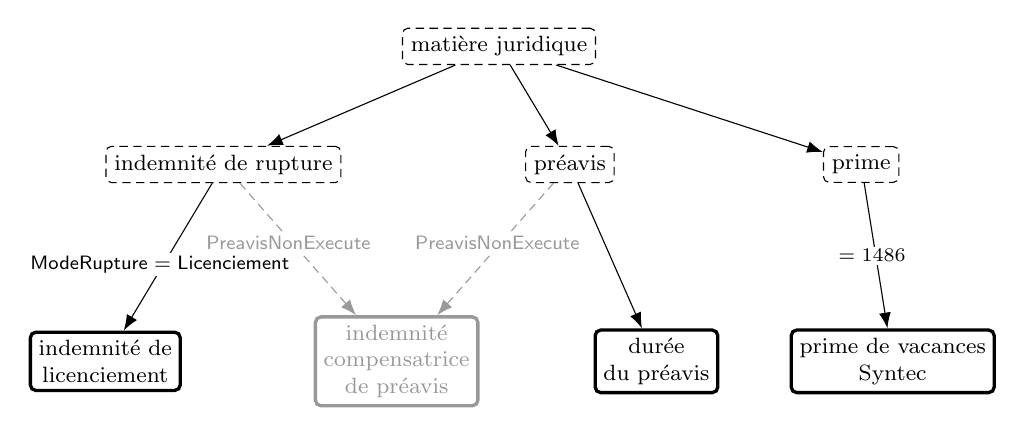
\begin{tikzpicture}[
  x=1cm, y=1cm,
  abs/.style={draw, rounded corners=2pt, align=center, font=\footnotesize,
    inner sep=3pt, densely dashed},
  conc/.style={draw, rounded corners=2pt, align=center, font=\footnotesize,
    inner sep=3pt, very thick},
  off/.style={conc, draw=elague, text=elague},
  arr/.style={-{Latex[length=2mm]}},
  offarr/.style={-{Latex[length=2mm]}, draw=elague, densely dashed},
  pred/.style={font=\scriptsize, align=center, fill=white, inner sep=1pt},
  offpred/.style={pred, text=elague}
]
\node[abs] (top) at (0,0) {matière juridique};
\node[abs] (rup) at (-3.5,-1.5) {indemnité de rupture};
\node[abs] (pre) at (0.9,-1.5) {préavis};
\node[abs] (pri) at (4.6,-1.5) {prime};
\node[conc] (lic) at (-5.0,-4.0) {indemnité de\\ licenciement};
\node[off] (icp) at (-1.3,-4.0) {indemnité\\ compensatrice\\ de préavis};
\node[conc] (dur) at (2.0,-4.0) {durée\\ du préavis};
\node[conc] (pvs) at (5.0,-4.0) {prime de vacances\\ Syntec};
\draw[arr] (top) -- (rup);
\draw[arr] (top) -- (pre);
\draw[arr] (top) -- (pri);
\draw[offarr] (rup) -- node[offpred, pos=0.45]{\(\PreavisNE\)} (icp);
\draw[offarr] (pre) -- node[offpred, pos=0.45]{\(\PreavisNE\)} (icp);
\draw[arr] (rup) -- node[pred, pos=0.55]{\(\ModeRupture=\mathsf{Licenciement}\)} (lic);
\draw[arr] (pre) -- (dur);
\draw[arr] (pri) -- node[pred]{\(\IDCC=1486\)} (pvs);
\end{tikzpicture}
\caption{Extrait d'une hiérarchie des matières. Les matières abstraites sont
  en pointillés, les matières concrètes en gras ; les arêtes sans étiquette
  portent le prédicat \(\true\), et l'indemnité compensatrice de préavis a deux
  parents. Pour le dossier fil rouge, l'indemnité de licenciement est établie
  et l'indemnité compensatrice écartée (en gris), le préavis ayant été
  exécuté.}
\label{fig:hierarchie}
\end{figure}

\paragraph{Exemple.} Dans le dossier fil rouge, la question porte sur une
matière abstraite, l'indemnité de rupture \(\IndemRupture\)
(figure~\ref{fig:hierarchie}). Le dossier indique que la rupture est un
licenciement, \(\ModeRupture=\mathsf{Licenciement}\), et que le préavis a été
exécuté, \(\PreavisNE=\false\) ; ainsi, dans l'extrait de la figure,
\(\Ouv_D(\IndemRupture)=\{\Indem\}\), et cette matière est établie. C'est
l'arbre de cette seule matière qui est saisi dans le dossier.

\subsection{Arbres à arêtes prédicatives}

\begin{defi}[Arbre normatif]\label{def:normative-tree}
Pour une matière \(m\), un \emph{arbre normatif} \(\theta\in\mc T(m)\) est un
quintuplet \(\theta=(V,E,r,\lambda,\pi)\) où \((V,E)\) est un arbre fini
enraciné, de racine \(r\in V\), dont les arêtes sont orientées du père vers
le fils, et
\[
 \lambda:V\setminus\{r\}\to\Cand_m,\qquad
 \pi:E\to\{\text{prédicats d'applicabilité}\}.
\]
On note \(\pi(e)(D):=\sem{\pi(e)}_D\). Pour \(e\in E\), soit
\(\dep(e):=\dep(\pi(e))\) ; pour \(u\in V\setminus\{r\}\) tel que
\(\sigma_{\lambda(u)}=(m_0,\ldots,m_n)\to m\), soit
\(\dep(u):=\{m_0,\ldots,m_n\}\) ; et
\[
 \dep(\theta):=\bigcup_{e\in E}\dep(e)\;\cup
                      \bigcup_{u\in V\setminus\{r\}}\dep(u).
\]
Pour \(u\in V\), on utilise comme d'habitude \(\child(u)\), \(\sib_u(v)\) et
\(\desc(v)\) (avec \(v\in\desc(v)\)) pour désigner respectivement les fils, les
frères et les descendants d'un nœud.
\end{defi}

Comme tout nœud autre que la racine possède exactement une arête entrante,
cette arête porte toutes les conditions d'applicabilité de son candidat, y
compris les conditions temporelles.

\paragraph{Exemple.} La figure~\ref{fig:arbre} représente l'arbre
\(\theta_{\Indem}\) du dossier fil rouge. Sous la racine, deux versions du Code
du travail s'excluent par leur date ; sous la version issue du décret de 2017
se trouvent les conventions de branche, chacune atteinte par un test sur
\(\IDCC\), et, pour Syntec, deux versions successives de la convention que la
date départage. Le candidat du Code est au-dessus des candidats conventionnels,
puisque \(\CodeTravail\normgt\AccordCollectif\) et par clôture par sous-typage
de l'ordre normatif. L'arête \(e\) qui mène à l'article 4.5 porte un prédicat
composé de deux tests :
\[
\begin{array}{l}
 \pi(e):=[\IDCC=1486]\land[\DateT\geq\text{1\textsuperscript{er} mai 2023}],\\
 \widehat \nu_D(\IDCC)= 1486,\quad
 \widehat \nu_D(\DateT)=\text{mars 2025}.
\end{array}
\]
Les deux tests sont établis, donc \(\pi(e)(D)=\true\), tandis que l'arête qui
mène à l'article~19, dont l'intervalle de dates se clôt le
1\textsuperscript{er}~mai 2023, vaut \(\false\)~\cite{frcode,syntec}. Si
\(\IDCC\) était indéfinie, \(\pi(e)(D)\) vaudrait \(\unknown\), et non
\(\false\) ; le prédicat de l'article~19 vaudrait encore \(\false\), son test
de date suffisant à l'exclure.

\begin{figure}
\centering
\begin{tikzpicture}[
  x=1cm, y=1cm,
  cand/.style={draw, rounded corners=2pt, align=center, font=\small,
    inner sep=3pt, minimum width=2.4cm},
  off/.style={cand, draw=elague, text=elague},
  sel/.style={cand, very thick},
  arr/.style={-{Latex[length=2mm]}, very thick},
  offarr/.style={-{Latex[length=2mm]}, draw=elague, densely dashed},
  pred/.style={font=\scriptsize, align=center, fill=white, inner sep=1pt},
  offpred/.style={pred, text=elague}
]
\node[cand] (r) at (0,0) {\(r\) : \(\Indem\)};
\node[off] (old) at (-3.4,-2.1) {Code du travail\\ rédaction antérieure};
\node[sel] (code) at (3.4,-2.1) {Code du travail, R.~1234-2\\
  {\scriptsize \(\ConvBranche\mapsto\Social\)}};
\draw[offarr] (r.south) -- ++(0,-0.45) -| (old.north);
\draw[arr] (r.south) -- ++(0,-0.45) -| (code.north);
\node[offpred] at (-3.4,-1.15) {\(\DateT<\text{27/09/2017}\)};
\node[pred] at (3.4,-1.15) {\(\DateT\geq\text{27/09/2017}\)};
\node[off] (s19) at (-5.1,-5.1) {Syntec, art.~19};
\node[sel] (s45) at (-1.7,-5.1) {Syntec, art.~4.5};
\node[off] (hcr) at (1.7,-5.1) {HCR};
\node[off] (met) at (5.1,-5.1) {Métallurgie};
\draw[offarr] (code.south) -- (3.4,-3.3) -| (s19.north);
\draw[offarr] (code.south) -- (3.4,-3.3) -| (hcr.north);
\draw[offarr] (code.south) -- (3.4,-3.3) -| (met.north);
\draw[arr] (code.south) -- (3.4,-3.3) -| (s45.north);
\node[offpred] at (-5.1,-4.15) {\(\IDCC=1486\)\\
  \(\DateT\in[\text{25/01/1996},\text{01/05/2023}[\)};
\node[pred] at (-1.7,-4.15) {\(\IDCC=1486\)\\ \(\DateT\geq\text{01/05/2023}\)};
\node[offpred] at (1.7,-4.15) {\(\IDCC=1979\)};
\node[offpred] at (5.1,-4.15) {\(\IDCC=3248\)};
\end{tikzpicture}
\caption{Arbre normatif \(\theta_{\Indem}\) de l'exemple fil rouge (le
  sous-arbre de la rédaction antérieure du Code et les rédactions de la
  convention Syntec antérieures à 1996 sont omis). Chaque arête porte son
  prédicat d'applicabilité. Pour le dossier de la section~\ref{sec:exemple},
  les branches grisées sont retirées par \((\Cut)\) et le chemin en gras est
  la forme normale de l'arbre. Le candidat du Code porte la politique
  \(\Social\) envers les conventions de branche.}
\label{fig:arbre}
\end{figure}

\subsection{Forêts normatives cohérentes}\label{sec:consistency}

Nous supposons que les arbres normatifs encodent fidèlement le contenu
calculatoire des textes qu'ils représentent ; le présent travail ne traite pas
de cette traduction. Nous imposons en revanche les conditions suivantes,
supposées dans toute la suite. Une \emph{forêt normative} est un ensemble fini
\(\mc F\subseteq\bigcup_{m\in\Matter}\mc T(m)\) contenant au plus un arbre par
matière ; on note \(\theta_m\) l'arbre de \(m\) lorsqu'il existe.

\begin{defi}[Cohérence]\label{def:consistency}
\(\mc F\) est \emph{cohérente} lorsque :
\begin{enumerate}
\item \emph{Les dépendances sont bien fondées.} Posons \(m'<_{\dep}m\) si et
  seulement si \(\theta_m\in\mc F\) et \(m'\in\dep(\theta_m)\). La relation
  \(<_{\dep}\) est acyclique.
\item Pour tout \(\theta_m=(V,E,r,\lambda,\pi)\in\mc F\) et tout dossier \(D\) :
\begin{enumerate}
\item \emph{Les arbres reflètent \(\normgt\).} Pour tous \(v,w\in V\setminus\{r\}\),
  \((v,w)\in E\Rightarrow s(\lambda(v))\normgt s(\lambda(w))\).
\item \emph{Les frères sont mutuellement exclusifs.} Pour
  \(v,v'\in\child(u)\) distincts, on n'a pas à la fois
  \(\pi((u,v))(D)=\true\) et \(\pi((u,v'))(D)=\true\).
\item \emph{La racine est exhaustive.} Il existe \(v\in\child(r)\) tel que
  \(\pi((r,v))(D)\neq\false\).
\item \emph{Les candidats sociaux sont comparables.} S'il existe
  \(u\in V\setminus\{r\}\) et \(s\in\Source\) tels que
  \(\widehat p(\lambda(u))(s)=\Social\), alors \(m\in\MatterOrd\).
\item \emph{Les politiques d'arbitrage sont totales sur le sous-arbre.} Pour
  tous \(u,v \in V\setminus\{r\}\),
  \(v \in \desc(u)\setminus\{u\} \Longrightarrow
  \widehat p(\lambda(u))
    \bigl(s(\lambda(v))\bigr)
  \neq \bot\).
\end{enumerate}
\item \emph{Les arbres portent sur des matières concrètes.} Pour tout
  \(\theta_m\in\mc F\), \(m\in\Matter_c\) ; et les prédicats de la hiérarchie
  ne portent que sur des matières sans arbre : pour toute arête \(e\) de la
  hiérarchie, \(\dep(\eta(e))\cap\mathrm{dom}(\mc F)=\emptyset\).
\end{enumerate}
\end{defi}

La condition~(b) fait d'une séparation horizontale un \emph{conflit} : un même
scénario factuel ne peut satisfaire à la fois deux prédicats frères
(exclusivité horizontale). Des frères peuvent représenter des conventions
collectives différentes ou des versions temporelles différentes d'un même
texte. Un candidat n'est jamais en conflit avec ses ancêtres, qui sont des
sources supérieures situées sur le même chemin. La condition~(c) garantit
qu'un arbre normatif contient toujours au moins un candidat applicable. Les conditions~(d) et~(e) assurent que les politiques
d'arbitrage sont toujours bien définies.

\section{Traitement des dossiers}\label{sec:op}

\subsection{Constructeurs}
Les dossiers sont construits et manipulés au moyen de quatre constructeurs,
que nous définissons à présent.
\begin{defi}[Constructeurs de dossiers]
Les constructeurs de dossiers sont
\[
\begin{array}{lll}
D &::=& \EmptyD \quad \text{le dossier vide}\\
&& \mid \Input(D,m,v)\quad m\in\Undef,\ v\in\Raw(m)\uplus\mc T(m)\\
&& \mid \Prune(D,m)\quad m\in\Unres \\
&& \mid \Resolve(D,m)\quad m\in\Unres.
\end{array}
\]
\end{defi}
Les applications de \(\Input\) à un arbre forment la forêt
\(\mc F_D:=\bigl(\nu_D(m)\bigr)_{m\in\Unres}\). Plus précisément,
\(\Input(D,m,\theta)\) ajoute un nouvel arbre \(\theta\in\mc T(m)\), indexé par
la matière nouvellement introduite \(m\), tandis que \(\Input(D,m,a)\), avec
\(a\in\Raw(m)\), ajoute une matière résolue mais aucun arbre. Des saisies
successives d'arbres pour des matières distinctes font donc apparaître
plusieurs arbres normatifs dans \(\mc F_D\).

Le dossier vide est \(\EmptyD=(\emptyset,[])\), où \([]\) désigne la valuation
vide. Pour \(D=(\mc M_D,\nu_D)\), on note \(\nu_D-m\) la valuation restreinte
\(\nu_D\mathrel\upharpoonright(\mc M_D\setminus\{m\})\), et
\(\nu_D+[m\mapsto v]\) l'extension de \(\nu_D\) par une nouvelle entrée
\(m\notin\mc M_D\) de valeur \(v\in\Raw(m)\uplus\mc T(m)\). Alors
\begin{equation}
\Input((\mc M_D,\nu_D),m,v)
 :=(\mc M_D\cup\{m\},\nu_D+[m\mapsto v]).
\label{eq:input}
\end{equation}
Cette opération ajoute un nouvel élément au dossier. La
section~\ref{sec:choix} y ajoute un opérateur de branchement, qui produit une
liste de dossiers.

\subsection{Élagage}

L'élagage est une relation de réécriture sur les arbres normatifs, indexée par
le dossier courant. Pour \(\theta=(V,E,r,\lambda,\pi)\) et
\(W\subseteq V\setminus\{r\}\) clos par descendants, on note
\(\theta\setminus W\) la restriction de \(\theta\) à \(V\setminus W\).

\begin{defi}[Réduction]\label{def:reduction}
Pour une arête \(e=(u,v)\in E\), on définit
\[
\begin{array}{lll}
 (\Cut) & \theta\redD\theta\setminus\desc(v)
   & \text{si }\pi(e)(D)=\false,\\[2pt]
 (\Select) & \theta\redD\theta\setminus\bigcup_{w\in\sib_u(v)}\desc(w)
   & \text{si }\pi(e)(D)=\true\text{ et }\sib_u(v)\neq\emptyset.
\end{array}
\]
\end{defi}

La règle \((\Cut)\) retire une arête dont le prédicat est faux ainsi que le
sous-arbre devenu inatteignable ; la règle \((\Select)\) retient la branche dont
le prédicat est établi et écarte ses frères.

\begin{prop}[Formes normales]\label{prop:norm}
Soit \(D\) un dossier dont la forêt \(\mc F_D\) est cohérente. Sur les arbres
de \(\mc F_D\) et leurs réduits, \(\redD\) termine et est confluente. Tout
\(\theta\in\mc F_D\) possède donc une unique forme normale, notée \(\nf\theta\).
\end{prop}
\begin{proof}
Terminaison : chaque pas retire un sommet d'un arbre fini. Pour la confluence
locale, on remarque que \(\pi(e)(D)\) ne dépend que de \(D\), et que des frères
dans un réduit sont frères dans \(\theta\), de sorte que~(b) vaut dans tout
réduit. Soient deux pas en \(e_i=(u_i,v_i)\), \(i=1,2\), qui retirent les
ensembles clos par descendants \(W_1,W_2\). Si \(v_2\in W_1\), alors
\(W_2\subseteq W_1\), et le pas en \(e_1\) soit s'applique encore dans
\(\theta_2\) et donne \(\theta_1\), soit est un \((\Select)\) dont les
sous-arbres frères sont tous inclus dans \(W_2\), auquel cas
\(\theta_1=\theta_2\). Si aucune des deux cibles n'appartient à l'ensemble de
l'autre, les deux pas s'appliquent encore et commutent. Le cas restant,
\(v_1\in W_2\) et \(v_2\in W_1\), force \(v_1\) et \(v_2\) à être frères avec
deux arêtes valant \(\true\), ce qu'exclut~(b). Le lemme de Newman permet de
conclure.
\end{proof}

\begin{equation}
\Prune((\mc M_D,\nu_D),m):=(\mc M_D,(\nu_D-m)+[m\mapsto\nf{\nu_D(m)}]).
\label{eq:prune}
\end{equation}

\begin{lemm}[Structure des formes normales]\label{lem:linear}
Soit \(\theta\in\mc T(m)\) un arbre d'une forêt cohérente et
\(\theta'=\nf\theta=(V',E',r,\lambda',\pi')\).
\begin{enumerate}
\item Si \(\pi(e)(D)\neq \unknown\) pour toute arête \(e\in E'\), alors
  \(\theta'\) est un chemin non vide \(r\to v_1\to\cdots\to v_k\) (\(k\geq1\))
  dont toutes les arêtes valent \(\true\), et
  \(s(\lambda(v_i))\normgt s(\lambda(v_{i+1}))\).
\item Si une arête \(e\in E'\) vérifie \(\pi(e)(D)=\unknown\), alors
  \(\dep(e)\cap(\Unres\cup\Undef)\neq\emptyset\).
\end{enumerate}
\end{lemm}
\begin{proof}
(1) Aucune arête de \(\theta'\) ne vaut \(\false\), sinon \((\Cut)\)
s'appliquerait ; toute arête vaut donc \(\true\). Si un nœud avait deux fils,
les deux arêtes vaudraient \(\true\), ce qui contredirait l'exclusion
mutuelle~(b) ; \(\theta'\) est donc un chemin. La racine conserve au moins un
fils par exhaustivité~(c) : son arête non fausse vaut \(\true\), et
\((\Select)\) a retiré les autres. La monotonie des sources découle de~(a).
(2) est la contraposée de la totalité
(définition~\ref{def:applicability-predicate}).
\end{proof}

\subsection{Interaction : ce que l'assistant doit demander}

Le lemme~\ref{lem:linear} identifie exactement ce qui bloque une résolution.
Pour \(\theta'=\nf{\nu_D(m)}=(V',E',r,\lambda',\pi')\), on définit
\[
 \NeedFacts_D(m):=\Bigl(\bigcup_{e\in E',\ \pi(e)(D)=\unknown}\dep(e)
   \;\cup\bigcup_{u\in V'\setminus\{r\}}\dep(u)\Bigr)
   \cap(\Unres\cup\Undef).
\]

Lorsque \(\NeedFacts_D(m)=\emptyset\), l'arbre est un chemin de candidats
exécutables et l'étape déterministe ci-dessous s'applique ; sinon, l'assistant
soumet \(\NeedFacts_D(m)\) à l'expert (pour les matières indéfinies) ou les
résout d'abord (pour les matières non résolues).

\paragraph{Exemple.} Tant que \(\IDCC\) est indéfinie, les arêtes qui mènent à
l'article 4.5, à HCR et à la métallurgie valent \(\unknown\), tandis que celle
de l'article~19 vaut déjà \(\false\), la date étant connue : \((\Cut)\) ne
retire que ce nœud, et \(\IDCC\in\NeedFacts_D(\Indem)\). Une fois \(\IDCC\)
saisie, l'élagage donne le chemin \(r\to c_{\mathsf{Code}}\to c_{4.5}\) de la
figure~\ref{fig:arbre}. Il reste alors \(\NeedFacts_D(\Indem)=\{\Categorie\}\),
puisque \(\Categorie\in\dep(c_{4.5})\) : c'est la question que l'assistant
pose ensuite, sous la forme d'un point de choix (section~\ref{sec:choix}).

\subsection{Résolution}\label{sec:resolution}

Soit \(\theta'=\nf{\nu_D(m)}\) un chemin \(r\to v_1\to\cdots\to v_k\) dont tous
les candidats sont exécutables, c'est-à-dire \(\dep(v_i)\subseteq\Res\). En
renversant le chemin, on obtient la liste des candidats par sources croissantes
\[
 L_D(m):=[c_0,\ldots,c_n]:=[\lambda(v_k),\ldots,\lambda(v_1)],\qquad
 s(c_0)\normlt\cdots\normlt s(c_n).
\]
Pour un candidat exécutable \(c\) tel que \(\sigma_c=(m_0,\ldots,m_q)\to m\),
sa valeur, obtenue sans modifier le dossier, est
\(D(c):=\phi_c(\nu_D(m_0),\ldots,\nu_D(m_q))\in\Raw(m)\).

\begin{defi}[Application récursive des politiques]\label{def:apply-policy}
Pour deux candidats \(a,b\in\Cand_m\) tels que \(s(a)\normlt s(b)\), on pose
\[
\Winner_D(a,b):=
\begin{cases}
 a,& \text{si } \widehat p(b)(s(a))=\Suppletive,\\
 a,& \text{si } \widehat p(b)(s(a))=\Social \text{ et } D(b)\fav{m}D(a),\\
 b,& \text{sinon,}
\end{cases}
\]
\[
 \ApplyPolicy_D([c]):=c,\qquad
 \ApplyPolicy_D(a::b::L):=\ApplyPolicy_D(\Winner_D(a,b)::L).
\]
Pour \(c^*:=\ApplyPolicy_D(L_D(m))\),
\begin{equation}
 \Resolve((\mc M_D,\nu_D),m):=(\mc M_D,(\nu_D-m)+[m\mapsto D(c^*)]).
 \label{eq:resolve}
\end{equation}
\end{defi}

\paragraph{Suite de l'exemple.}
Plaçons-nous dans le scénario où la salariée relève des ingénieurs et cadres :
\(\nu_D(\Categorie)=\Cadre\). Le chemin subsistant est
\(r\to c_{\mathsf{Code}}\to c_{4.5}\), soit
\(L_D(\Indem)=[c_{4.5},c_{\mathsf{Code}}]\), et
\[
\widehat p(c_{\mathsf{Code}})(\Syntec)=\Social
\quad\text{puisque}\quad \Syntec\subtype\ConvBranche.
\]
Le dossier donne
\[
\begin{array}{l}
\nu_D(\Salary)=\nu_D(\MoisRem)=3\,000\ \text{euros},\\
\nu_D(\Senior)=\nu_D(\Presence)=10\ \text{ans},
\end{array}
\]
et les deux candidats s'évaluent par leur code Catala
(figure~\ref{fig:catala}) : \(D(c_{\mathsf{Code}})=3\,000\times10\times\frac14
=7\,500\) euros par le premier cas de R.~1234-2, et
\(D(c_{4.5})=3\,000\times10\times\frac13=10\,000\) euros par le barème des
ingénieurs et cadres. Puisque \(D(c_{\mathsf{Code}})\fav{\Indem}D(c_{4.5})\),
le candidat conventionnel l'emporte (définition~\ref{def:apply-policy}) ; si la
politique du candidat du Code avait été \(\Absolute\), il aurait prévalu quels
que soient les montants. Si \(\Salary\) avait été indéfinie, on aurait eu
\(\NeedFacts_D(\Indem)=\{\Salary\}\), et l'assistant l'aurait demandée avant
toute comparaison.

Le corpus réalise cette comparaison dans un module distinct, qui met en œuvre
l'article L.~2251-1 (figure~\ref{fig:concours}) : un pli (\emph{fold}),
\texttt{combine},
part de la norme supérieure et ne la remplace par une source inférieure que si
le critère de faveur tient celle-ci pour plus favorable. Le corpus limite ce
concours à une seule source inférieure ; il calcule alors
\(\ApplyPolicy_D\) sous le régime \(\Social\), au traitement de l'égalité
près : à montants égaux, le corpus conserve la norme supérieure, là où la
définition~\ref{def:apply-policy} retient la source inférieure. La valeur
retenue est la même.

\begin{figure}
\begin{Verbatim}[frame=single, label={Code du travail, article L. 2251-1}]
champ d'application ConcoursIndemnitéDeLicenciement_Loi:
  définition la_plus_favorable égal à
    combine tout c parmi sources_inférieures dans meilleure
      initialement norme_supérieure avec
      (si (résultat de Critere.PlusFavorableAuSalarié_Loi avec {
            -- position_du_salarié: position_du_salarié
            -- grandeur_examinée:
              grandeur_de_l_indemnité_de_licenciement de c.réponse
            -- grandeur_de_référence:
              grandeur_de_l_indemnité_de_licenciement de meilleure.réponse
          }).l_examinée_est_plus_favorable
       alors c sinon meilleure)
\end{Verbatim}
\caption{Le concours de normes sous l'ordre public social dans le
  corpus~\cite{corpuslumo} : un pli qui part de la norme supérieure
  (commentaires omis, mise en page adaptée).}
\label{fig:concours}
\end{figure}

\begin{theo}[Résolution]\label{thm:resolution}
Soit \(D\) un dossier dont la forêt \(\mc F_D\) est cohérente et dont toutes
les dépendances figurent dans le dossier : \(\dep(\theta_m)\subseteq\mc M_D\)
pour tout \(m\in\Unres\). Il existe alors une suite finie de pas \(\Prune\) et
\(\Resolve\) menant à un dossier \(D'\) tel que \(\UnresOf{D'}=\emptyset\).
\end{theo}
\begin{proof}
Par récurrence sur \(|\Unres|\). S'il est nul, il n'y a rien à faire. Sinon,
\(<_{\dep}\) est acyclique et \(\Unres\) est fini ; on peut donc choisir
\(m\in\Unres\) minimal pour \(<_{\dep}\) parmi \(\Unres\). Aucun
\(m'\in\Unres\) n'appartient à \(\dep(\theta_m)\) ; avec l'hypothèse,
\(\dep(\theta_m)\subseteq\Res\). Par totalité, toute arête de \(\theta_m\) est
décidée ; d'après le lemme~\ref{lem:linear}, \(\nf{\theta_m}\) est donc un
chemin non vide dont les candidats ont toutes leurs entrées dans \(\Res\), et
sont donc exécutables. Ainsi \(\Resolve(\Prune(D,m),m)\) est défini et fait
passer \(m\) parmi les matières résolues sans modifier aucun autre arbre, ce qui fait
strictement décroître \(|\Unres|\). La cohérence et l'hypothèse sur les
dépendances sont préservées, puisqu'aucun arbre n'a été ajouté.
\end{proof}

\begin{coro}[Boucle interactive]\label{cor:loop}
Soit \(\mc F\) une forêt finie cohérente (le référentiel) et
\(\mathrm{dom}(\mc F)\) l'ensemble des matières qui possèdent un arbre dans
\(\mc F\). Partons d'un dossier dont tous les arbres appartiennent à \(\mc F\),
et supposons que l'expert réponde à toute demande portant sur une matière
indéfinie \(m\) soit par une valeur brute, soit par \(\theta_m\in\mc F\)
lorsque \(m\in\mathrm{dom}(\mc F)\). La boucle qui, de façon répétée,
(i)~choisit \(m\in\Unres\) minimal pour \(<_{\dep}\), (ii)~élague, puis
(iii)~demande \(\NeedFacts_D(m)\) s'il est non vide et résout \(m\) sinon,
termine avec \(\Unres=\emptyset\) après au plus \(|\mathrm{dom}(\mc F)|\)
saisies d'arbres. La suite des saisies et des pas constitue un journal de la
résolution.
\end{coro}
\begin{proof}
À chaque étape, \(\mc F_D\subseteq\mc F\) à l'élagage près, donc \(\mc F_D\)
est cohérente : \(<_{\dep}\) restreinte à une sous-forêt reste acyclique et les
conditions portant sur chaque arbre sont héritées. Par minimalité de \(m\),
aucune matière de \(\Unres\) n'appartient à \(\dep(\theta_m)\) ; on a donc
\(\NeedFacts_D(m)\subseteq\Undef\), et l'étape~(iii) est bien définie. Lorsque
\(\NeedFacts_D(m)=\emptyset\), toutes les arêtes de \(\nf{\theta_m}\) sont
décidées et ses candidats sont exécutables, si bien que \(\Resolve\) s'applique
comme dans le théorème~\ref{thm:resolution}. Toute matière demandée appartient
à \(\dep(\mc F):=\bigcup_{\theta\in\mc F}\dep(\theta)\), qui est fini. Soit
\(I_D\) l'ensemble (croissant) des matières pour lesquelles un arbre a déjà
été saisi. Le triplet
\[
 \bigl(|\mathrm{dom}(\mc F)\setminus I_D|,\;
       |\dep(\mc F)\setminus\mc M_D|,\;
       |\Unres|\bigr)
\]
décroît lexicographiquement à chaque itération : une saisie d'arbre fait
décroître la première composante ; une saisie de valeur laisse la première
inchangée et fait décroître la deuxième ; un pas \(\Resolve\) laisse les deux
premières inchangées et fait décroître la troisième. La boucle termine donc,
et elle ne peut s'arrêter qu'avec \(\Unres=\emptyset\).
\end{proof}

Dans l'exemple, les matières d'ancienneté et de salaire ont été saisies comme
valeurs brutes. Dans le corpus, ce sont des matières dotées de leurs propres
arbres, inférieures à \(\Indem\) pour \(<_{\dep}\), donc résolues avant elle.
Le prototype d'\ALex{} suit cet ordre : le corpus déclare, pour chaque champ,
les valeurs qu'il lit et le champ qui les produit, et \ALex{} exécute les
producteurs avant les consommateurs, c'est-à-dire dans l'ordre de
\(<_{\dep}\).

\paragraph{Ouverture des matières.} Lorsque la question porte sur une matière
abstraite \(m\), l'assistant commence par l'ouvrir. Tant qu'une matière de
\(\Ouv_D(m)\) est en suspens, il demande les matières des prédicats de la
hiérarchie qui valent \(\unknown\), auxquelles l'expert répond par une valeur
brute ; puis il saisit, par \(\Input\), l'arbre de chaque matière établie qui
en possède un. Chaque demande définit une nouvelle matière de l'ensemble fini
\(\bigcup_e\dep(\eta(e))\) : cette phase termine, et la boucle du
corollaire~\ref{cor:loop} prend le relais. Les demandes de cette phase
peuvent, elles aussi, être posées comme des points de choix, par exemple
lorsque le mode de rupture est discuté.

\subsection{Valeurs en conflit et branchement}\label{sec:choix}

Dans la boucle du corollaire~\ref{cor:loop}, l'expert répond à chaque demande
par une valeur unique. Un fait peut pourtant être incertain, et une
qualification discutée : la salariée de l'exemple se dit cadre, son employeur
la range parmi les ETAM. L'avocat construit alors une demande principale et des
demandes subsidiaires, chacune fondée sur une autre valeur. Plutôt que de
trancher, le dossier enregistre le conflit, et l'évaluation branche sur
chacune de ses valeurs.

\begin{defi}[Valeurs en conflit]\label{def:conflit}
Pour une matière concrète \(m\), on note \(a_1\conflit\cdots\conflit a_k\),
\(k\geq1\), une suite finie de valeurs deux à deux distinctes de \(\Raw(m)\), et
\(\Raw(m)^{\conflit}\) l'ensemble de ces suites. Nous étendons les valuations,
\[
\nu_D:\prod_{m\in\mc M_D}\bigl(\Raw(m)^{\conflit}\uplus\mc T(m)\bigr),
\]
et \(\Input(D,m,v)\) accepte désormais \(v\in\Raw(m)^{\conflit}\uplus\mc
T(m)\). Une matière est résolue lorsque sa valuation est une valeur seule
(\(k=1\)), et \emph{en conflit} lorsque \(k\geq2\) ; on note \(\Conf\)
l'ensemble des matières en conflit.
\end{defi}

À l'ordre d'écriture près, qui fixe l'ordre des scénarios, \(\nu_D(m)\) est
ainsi l'ensemble des valeurs possibles de \(m\), toutes en conflit, et une
matière indéfinie est une matière sans valeur possible. Une matière en conflit
n'a pas de valeur établie : \(\widehat\nu_D(m)=\bot\), les tests qui la lisent
valent \(\unknown\), et elle entre dans \(\NeedFacts_D\) : dans sa définition
comme dans le lemme~\ref{lem:linear}, \(\Unres\cup\Undef\) est désormais
remplacé par \(\Unres\cup\Undef\cup\Conf\).
Les résultats précédents valent pour les dossiers sans conflit. Le \emph{point
de choix} est la demande par laquelle l'assistant fait appel à l'utilisateur,
qui répond par \(a_1\conflit\cdots\conflit a_k\) : la valeur \(a_1\) est
\emph{retenue} (\(+\)), les suivantes sont des \emph{réserves} (\(-\)), et les
valeurs admissibles non citées sont \emph{écartées} (\(!\)). Le choix est
\emph{exclusif} si \(k=1\), et \emph{inclusif} sinon.

\begin{defi}[Branchement]\label{def:brancher}
Pour \(m\in\Conf\) de valuation \(a_1\conflit\cdots\conflit a_k\), on pose
\[
\Brancher(D,m):=[\,D[m:=a_1],\ \ldots,\ D[m:=a_k]\,],
\]
où \(D[m:=a]:=(\mc M_D,(\nu_D-m)+[m\mapsto a])\).
\end{defi}

La boucle interactive s'étend aux listes de dossiers. À l'étape~(iii),
l'assistant traite les matières requises une à une, dans un ordre fixé :
d'abord celles des arêtes qui valent \(\unknown\), puis les entrées des
candidats subsistants, en élaguant l'arbre de nouveau après chaque étape. Une
matière indéfinie est demandée par un point de choix ; une matière en conflit
est branchée, et la boucle poursuit le premier dossier de la liste en plaçant
les autres à sa suite. Le branchement est donc paresseux : un conflit sur une
matière qu'aucun prédicat ni aucun candidat subsistant ne lit ne crée aucun
scénario. Un dossier sans conflit dont toutes les matières sont résolues est un
\emph{scénario}. L'exécution décrit un \emph{arbre de décision} dont chaque
nœud est un branchement, dont les fils sont ordonnés comme les valeurs en
conflit, et dont les feuilles sont les scénarios.

\begin{prop}[Scénarios]\label{prop:scenarios}
Sous les hypothèses du corollaire~\ref{cor:loop}, supposons que l'utilisateur
réponde à chaque demande par une valeur, éventuellement en conflit, ou par un
arbre de \(\mc F\). La boucle étendue termine alors. Elle produit une liste
finie \([C_1,\ldots,C_n]\), \(n\geq1\), de scénarios, ordonnée selon l'ordre
lexicographique des rangs des valeurs le long des chemins de l'arbre de
décision : \(C_1\) est le scénario principal, \(C_2,\ldots,C_n\) sont les
scénarios subsidiaires.
\end{prop}
\begin{proof}
Le long d'un chemin de l'arbre de décision, le quadruplet formé des trois
composantes de la mesure du corollaire~\ref{cor:loop}, la dernière précédée de
\(|\Conf|\), décroît lexicographiquement : une saisie fait décroître l'une des
deux premières composantes, un branchement laisse celles-ci inchangées et fait
décroître \(|\Conf|\), et un pas \(\Resolve\) ne fait décroître que
\(|\Unres|\). Chaque chemin est donc fini, et se termine sur un scénario.
Chaque nœud a un nombre fini de fils. Un arbre à branchement fini dont tous les
chemins sont finis est fini (lemme de König) ; le parcours en profondeur,
réserves après valeur retenue, énumère ses feuilles dans l'ordre
lexicographique.
\end{proof}

C'est l'exploration que réalise le gestionnaire de scénarios du prototype
d'\ALex{} : après une sélection finale complète, il remonte à la réserve non
épuisée la plus profonde, conserve le préfixe des décisions qui la précèdent,
puis recalcule la suite.

\begin{remark}[Conflits d'interprétation]
On pourrait aussi admettre des arbres en conflit,
\(\nu_D(m)=\theta_1\conflit\theta_2\), pour deux lectures d'un même régime,
par exemple lorsque la qualification d'ordre public d'un texte est discutée.
Ce cas se ramène au précédent. On ajoute une matière factuelle \(I_m\) de
domaine \(\{1,2\}\) et l'on fusionne les deux arbres sous une même racine, en
conjoignant le test \([I_m=i]\) au prédicat de chaque arête issue de la racine
de \(\theta_i\) : la cohérence est préservée, et
\(\nu_D(I_m)=1\conflit2\) fait brancher l'élagage sur les deux lectures. Nous
ne branchons donc que sur des valeurs.
\end{remark}

\paragraph{Exemple.}
Dans le dossier fil rouge (figure~\ref{fig:decision}), l'assistant demande
d'abord \(\IDCC\) ; l'entreprise relève sans discussion de la convention
Syntec, et la réponse \(1486\) est exclusive. Après l'élagage,
\(\Categorie\in\NeedFacts_D(\Indem)\) : la salariée revendique la qualité de
cadre et invoque, à titre subsidiaire, sa classification d'ETAM. Le dossier
\(D'\) obtenu enregistre ce conflit :
\[
\nu_{D'}(\Categorie)=\Cadre\conflit\Etam.
\] Comme \(c_{4.5}\) lit la
catégorie, la boucle calcule \(\Brancher(D',\Categorie)\), qui produit deux
scénarios. Dans \(C_1\), la résolution de la section~\ref{sec:resolution} donne
10\,000 euros au titre de l'article 4.5. Dans \(C_2\), le barème des ETAM
jusqu'à dix ans d'ancienneté donne \(3\,000\times10\times\frac14=7\,500\)
euros, montant égal au plancher légal. Le montant est donc de 7\,500 euros quel
que soit le candidat sélectionné : la définition~\ref{def:apply-policy}
sélectionne \(c_{4.5}\), le corpus conserverait le Code. La demande principale
porte donc sur 10\,000 euros, la demande subsidiaire sur 7\,500 euros.

\begin{figure}
\centering
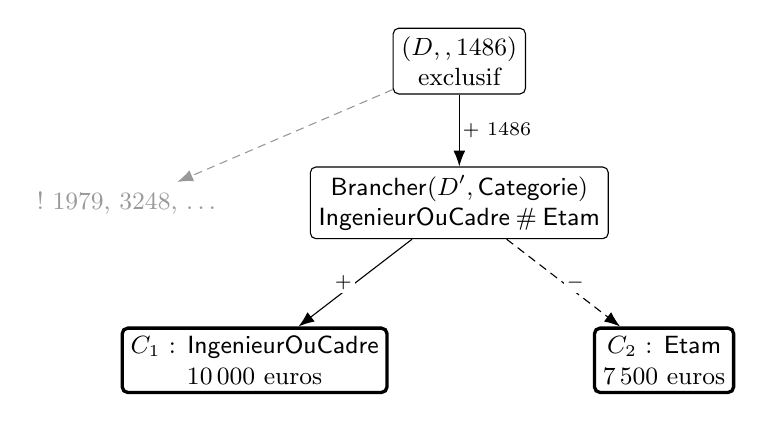
\begin{tikzpicture}[
  font=\small,
  q/.style={draw, rounded corners=2pt, align=center, inner sep=3pt},
  leaf/.style={draw, rounded corners=2pt, align=center, inner sep=3pt, very thick},
  arr/.style={-{Latex[length=2mm]}},
  offarr/.style={-{Latex[length=2mm]}, draw=elague, densely dashed},
  lab/.style={font=\scriptsize, fill=white, inner sep=1pt}
]
\node[q] (q1) at (0,0) {\(\Input(D,\IDCC,1486)\)\\ exclusif};
\node[text=elague] (x1) at (-4.2,-1.8) {\(!\)\ 1979, 3248, \ldots};
\node[q] (q2) at (0,-1.8) {\(\Brancher(D',\Categorie)\)\\
  \(\Cadre\conflit\Etam\)};
\node[leaf] (c1) at (-2.6,-3.8) {\(C_1\) : \(\Cadre\)\\ 10\,000 euros};
\node[leaf] (c2) at (2.6,-3.8) {\(C_2\) : \(\Etam\)\\ 7\,500 euros};
\draw[arr] (q1) -- node[lab, right]{\(+\)\ 1486} (q2);
\draw[offarr] (q1) -- (x1);
\draw[arr] (q2) -- node[lab, left]{\(+\)} (c1);
\draw[arr, densely dashed] (q2) -- node[lab, right]{\(-\)} (c2);
\end{tikzpicture}
\caption{Arbre de décision du dossier fil rouge : une saisie exclusive de
  \(\IDCC\), puis un branchement sur la catégorie, en conflit. La valeur
  retenue (\(+\)) donne le scénario principal \(C_1\), la réserve (\(-\)) le
  scénario subsidiaire \(C_2\) ; les valeurs écartées (\(!\)) ne sont pas
  explorées.}
\label{fig:decision}
\end{figure}

\section{Conclusion}\label{sec:conclusion}

Le modèle développé dans cet article isole une étape du calcul juridique
souvent laissée implicite : la sélection de la règle habilitée à effectuer le
calcul. Il représente les règles juridiques exécutables comme des candidats
typés par matière, les organise en arbres normatifs ordonnés par les sources et
à arêtes prédicatives, et utilise des tests d'applicabilité trivalués pour
distinguer les branches exclues de celles auxquelles il manque seulement de
l'information. Il fournit ainsi la base d'un assistant interactif capable de
demander les éléments manquants d'un dossier, d'élaguer l'arbre en
conséquence, puis d'appliquer les politiques d'arbitrage pertinentes pour
sélectionner un calcul exécutable. La hiérarchie des matières sépare la
question de savoir si une matière se pose de celle de savoir quelle règle y
répond, et garantit que le principe de faveur ne compare que des calculs d'une
même matière. Les valeurs en conflit et l'opérateur de branchement
permettent à l'assistant de faire appel à l'utilisateur lorsqu'un fait ou une
qualification est discuté, et d'en tirer un scénario principal et des
scénarios subsidiaires. Le théorème de
résolution montre que, sous des hypothèses de cohérence et d'acyclicité des
dépendances, ce processus finit par résoudre toutes les matières du dossier, et
la proposition~\ref{prop:scenarios} étend ce résultat aux scénarios. L'exemple
fil rouge illustre enfin l'application du modèle à du code Catala existant :
chaque champ qui calcule la matière devient un candidat, et le régime
d'articulation que le corpus laisse hors du code devient la politique du
candidat. C'est
l'architecture d'\ALex{}.

Plusieurs extensions rapprocheraient ce modèle de la structure du raisonnement
juridique tel qu'il se pratique. D'abord, le référentiel devrait aussi contenir
des règles juridiques non calculatoires. De telles règles auraient leurs
propres sources et leurs propres conditions temporelles d'applicabilité, mais
définiraient des politiques plutôt que des valeurs. En effet, la politique qui
gouverne l'articulation de deux calculs n'est pas nécessairement énoncée dans
l'un ou l'autre des textes qui les définissent : elle peut être fixée par une
troisième disposition, de rang supérieur~\cite{moizard2025fragmentation}.
L'article 4.5 de la convention Syntec offre le cas inverse : c'est la source
inférieure qui y énonce la règle de sélection, puisque « l'employeur verse
l'indemnité dont le montant est le plus élevé » entre l'indemnité
conventionnelle et l'indemnité légale, clause que le corpus n'encode pas
encore.
Représenter explicitement ces dispositions permettrait de distinguer la
provenance d'un calcul de celle de la règle qui gouverne son articulation avec
d'autres calculs.

Ensuite, l'élagage devrait être doté d'une sémantique formelle de provenance.
Outre l'arbre subsistant, la procédure devrait renvoyer un objet de
dérivation qui enregistre les branches neutralisées et les raisons de leur
exclusion : quels prédicats ont été évalués, quelles valeurs du dossier ont été
utilisées, et quelles comparaisons de politiques ont déterminé le résultat. Une
telle trace fournirait la matière nécessaire au contrôle de la résolution et à
sa transformation en une explication juridiquement signifiante.

Enfin, l'ordre des scénarios est aujourd'hui celui des réponses de
l'utilisateur. Le confronter aux valeurs obtenues permettrait de signaler une
réserve qui ne change pas le montant retenu : au-delà de dix ans d'ancienneté,
la convention Syntec applique le même taux aux ETAM et aux cadres, et la
demande subsidiaire de notre exemple deviendrait sans objet.

\paragraph{Remerciements.}
Des outils d'IA générative ont été utilisés comme suit. OpenAI GPT-5 a
relevé une incohérence de notre définition des politiques d'arbitrage au regard
du droit français. Claude Fable 5.1 (Anthropic) a été utilisé au fil des
versions successives pour relire les définitions formelles et les
démonstrations, proposer des formulations plus compactes des
définitions~\ref{def:types} et~\ref{def:favorable} et de l'une des conditions
de cohérence, et suggérer des références bibliographiques manquantes. Tous les
textes et références produits par IA ont été vérifiés, corrigés et validés par
les auteurs. Le modèle, les définitions et les résultats sont ceux des auteurs.

\bibliographystyle{alpha-fr}
\bibliography{references-fr}

\end{document}
